\documentclass[12pt]{article}
%\documentclass{article}

\usepackage{times}
\usepackage[final]{graphicx}
\usepackage{hyperref}

\setlength{\topmargin}{-0.5in}
\setlength{\oddsidemargin}{0in}
\setlength{\evensidemargin}{0in}
\setlength{\textwidth}{6.5in}
\setlength{\textheight}{9.0in}

\begin{document}

\centerline{\bf \Large CS295/CS395/CSYS395: \href{CS295_395_Syllabus.pdf}{\underline{Evolutionary Robotics}}}

\vspace{0.5cm}

\centerline{\bf \large Programming Assignment 5 of 10}

\vspace{0.5cm}

\centerline{\large Assigned: Friday, September 30, 2011}

\vspace{0.5cm}

\centerline{\large Due: Friday, October 7, 2011 by midnight}

\vspace{0.5cm}

\noindent \textbf{Description:} In this assignment you will start with the `empty' simulation you created in assignment 4 and incrementally add objects to construct a quadrupedal robot. In the next assignment you will add joints to your simulation so that the objects are connected together, then sensors, then motors, and then a controlling neural network.

\begin{enumerate}

\item Create a directory, Assignment\_4, that contains your assignment 4 submitted document. Move the ode-0.11.1 directory into this directory as well. Back up this directory. Now in subsequent assignments if you find your simulation becomes unusable you can go back and retrieve the `empty' simulation stored in this directory.

\item Create a new directory, Assignment\_5, and copy the ode-0.11.1 directory here. For the remainder of this assignment make changes to the files in this ode directory.

\item Draw the image shown in Fig. \ref{Fig1} on a blank sheet of paper. Draw to fill an entire page, as you will be annotating the image through the next few assignments.

\begin{figure}[!t]
\centerline{
\includegraphics[width=1.0\textwidth]{Robot_Schematic}
}
\caption{A template for sketching the quadrupedal robot to be simulated.}
\label{Fig1}
\end{figure}

\item Now draw the robot from the three additional perspectives as we did in class.

\item For the four upper and four lower legs, mark their positions, sizes (radius and length) and orientations (see Lecture 6, slide 4) in the three panels. You can choose the lengths and radii of the legs to your liking.

\item Now, in the empty demo\_buggy program, we need to create body and geom data structures to store all the objects that make up the robot. Replace

\texttt{static dWorldID world;}\\
\texttt{static dSpaceID space;}\\
\texttt{static dBodyID body[4];}\\
\texttt{static dJointID joint[3];	// joint[0] is the front wheel}\\
\texttt{static dJointGroupID contactgroup;}\\
\texttt{static dGeomID ground;}\\
\texttt{static dSpaceID car\_space;}\\
\texttt{static dGeomID box[1];}\\
\texttt{static dGeomID sphere[3];}\\
\texttt{static dGeomID ground\_box;}\\
    with \\
\texttt{static dWorldID world;}\\
\texttt{static dSpaceID space;}\\
\texttt{static dJointGroupID contactgroup;}\\
\texttt{static dBodyID body[9]; // one main body, 4x2 leg segments}\\
\texttt{static dGeomID geom[9];\\
static dGeomID ground;}\\

\item Recompile the code. If you get errors, delete those parts of the code that refer to the variables you deleted. Continue this process until you compile and run without errors.

\item Now you will create some functions that can be used to add objects to the empty simulator. Create a function of the form \\
\texttt{void CreateBox(	int index,}\\
\texttt{				double x, double y, double z,}\\
\texttt{				double length, double width, double height) \{}\\
\texttt{	...}\\
\texttt{	body[index] = ...}\\
\texttt{	...}\\
\texttt{	geom[index] = ...}\\
\texttt{	...}\\
\texttt{\}} \\
which will be used to create the main body of the robot. Refer to the commented-out code to figure out how to create an object. Assume the mass of all objects for now is 1. Without calling the function, recompile and run until you have no errors.

\item Create a similar function for creating cylinders, which will be used to create the upper and lower legs of the robot. You will need to add additional parameters for specifying the orientation of the cylinder. Recompile and run until error-free.

\item Create another function \\
\texttt{void DeleteObject( int index ) \{}\\
\texttt{	...}\\
\texttt{\}} \\
which can be used to remove objects from the simulation. This function should destroy both the body and the geom associated with the object using \texttt{dBodyDestroy} and \texttt{dGeomDestroy}. Recompile and run until error-free.

\item Now, in the main function, add code to create the first object, simulate the `robot', and delete the first object when the simulation terminates:\\
\texttt{CreateBox(...);}\\
\texttt{dsSimulationLoop (argc,argv,352,288,\&fn);}\\
\texttt{DeleteObject(...);}\\
Compile and run until error-free. Note that you will not see the object; why?

\item Two reasons: The simLoop function is commented out, and we have not specified that the object should be drawn, only simulated. Uncomment \\
\texttt{dSpaceCollide (space,0,\&nearCallback);}\\
\texttt{dWorldStep (world,0.05);}\\
\texttt{dJointGroupEmpty(contactgroup);}\\
in simLoop, recompile and run.

\item Create a new function \texttt{DrawBox(int index)} that will draw a box defined by \texttt{body[index]} and \texttt{geom[index]}. Refer to the code commented out at the bottom of \texttt{simLoop} to see how to do this. Without calling the new function, compile and run until error-free.

\item Add a line at the bottom of simLoop \\
\texttt{DrawBox(0);}\\
that will draw the first object during each pass through simLoop. Recompile and, when run, you should see the box fall and come to rest on the ground as in Fig. \ref{Fig2}a. (You can toggle texture drawing using CTRL-t.) Screencapture this image and paste into your document.

\item The object will have fallen too fast for you to follow it with your eyes. In order to start simulations paused and then step through them, modify simLoop to\\
\texttt{if ( !pause ) \{}\\
\texttt{dSpaceCollide (space,0,\&nearCallback);}\\
\texttt{dWorldStep (world,0.05);}\\
\texttt{dJointGroupEmpty(contactgroup);}\\
\texttt{\}}\\
\texttt{DrawBox(0);}\\

\item When you run test\_buggy, add \texttt{-pause} to start the program paused. Consult your compiler's documentation to determine how to add command arguments. When you re-run the program you should see the box hanging in midair as in Fig. \ref{Fig2}b. Screencapture and paste into your document. CTRL-o will advance the simulation by one time step; CTRL-p will unpause the simulation and cause the object to fall to the ground.

\item Add \texttt{CreateCylinder(1,...)} before simLoop is called, \texttt{DeleteObject(1)} after simLoop ends, and \texttt{DrawCylinder(1)} within simLoop to add the next object to the robot. Note that you will have to specify the orientation of the cylinder, which you do not have to do for the main body. When run in paused mode you should see both objects as in Fig. \ref{Fig2}c. Screencapture and copy and paste into your document.

\item Add a third object, compile, run and ensure that the object appears where you expect it. Continue to add an object and recompile until all nine objects are added. This should produce a simulation as shown in Fig. \ref{Fig2}d. Screencapture, copy and paste into your document, and submit.
\end{enumerate}

\begin{figure}[!t]
\centerline{
a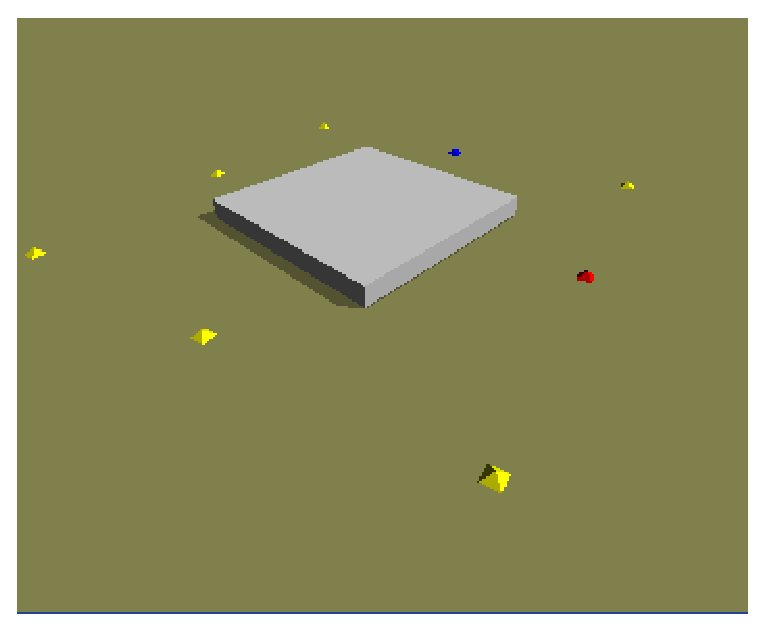
\includegraphics[width=0.4\textwidth]{Fig2a}
b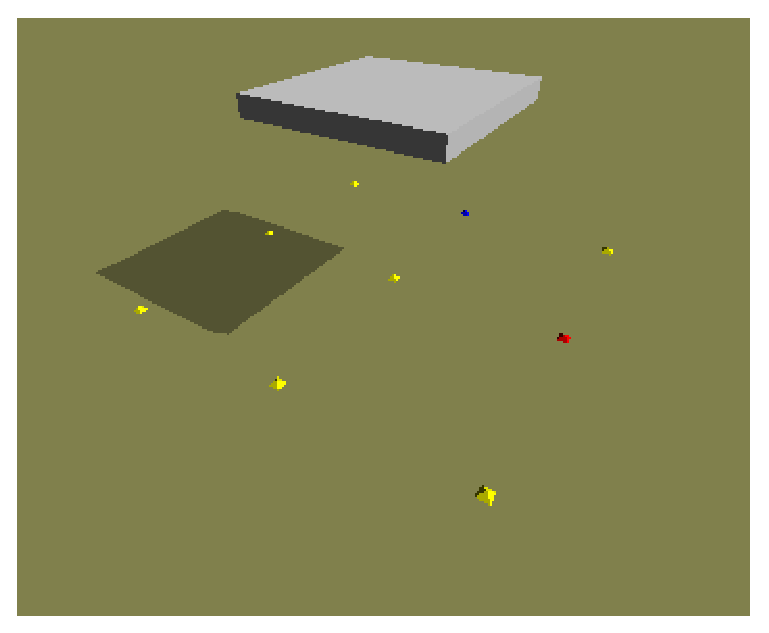
\includegraphics[width=0.4\textwidth]{Fig2b}
}
\centerline{
c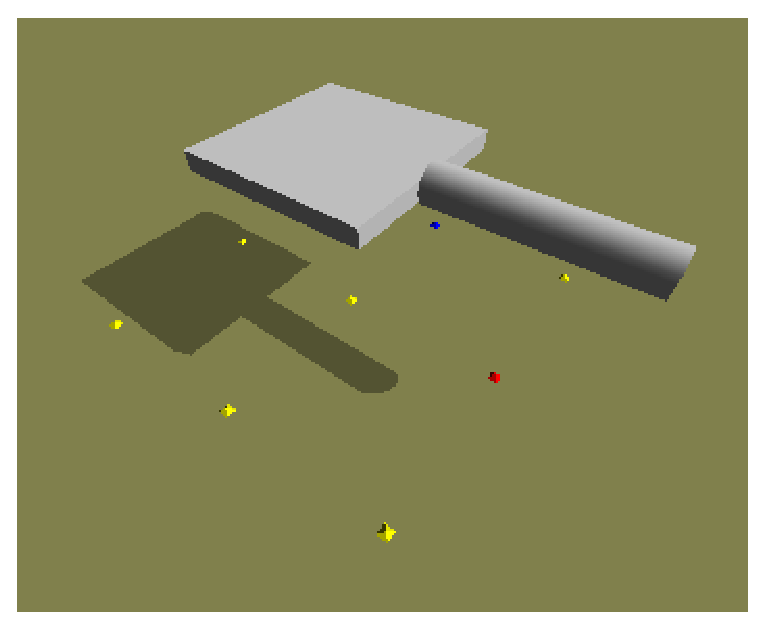
\includegraphics[width=0.4\textwidth]{Fig2c}
d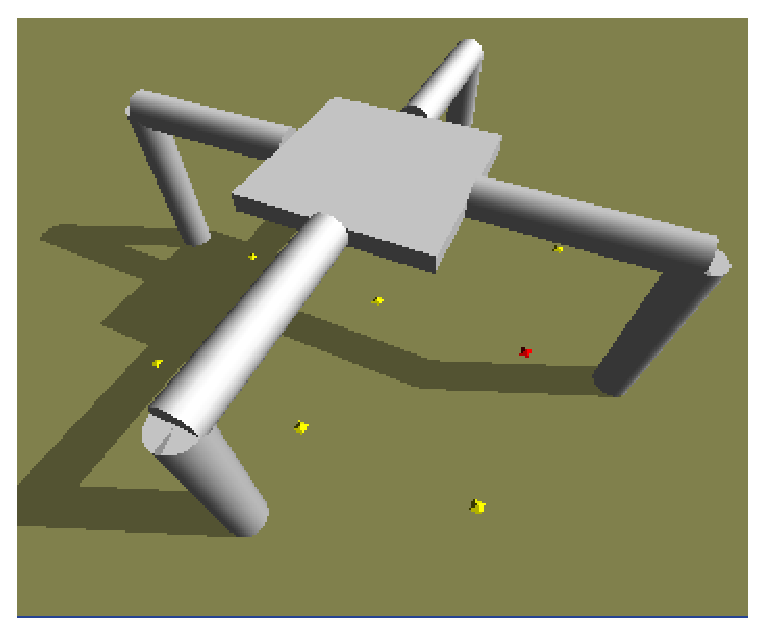
\includegraphics[width=0.4\textwidth]{Fig2d}
}
\caption{The quadrupedal robot under construction in ODE.}
\label{Fig2}
\end{figure}

\end{document} 
